\subsection{Experimental Setup}
\begin{figure}[!t]
  \centering
  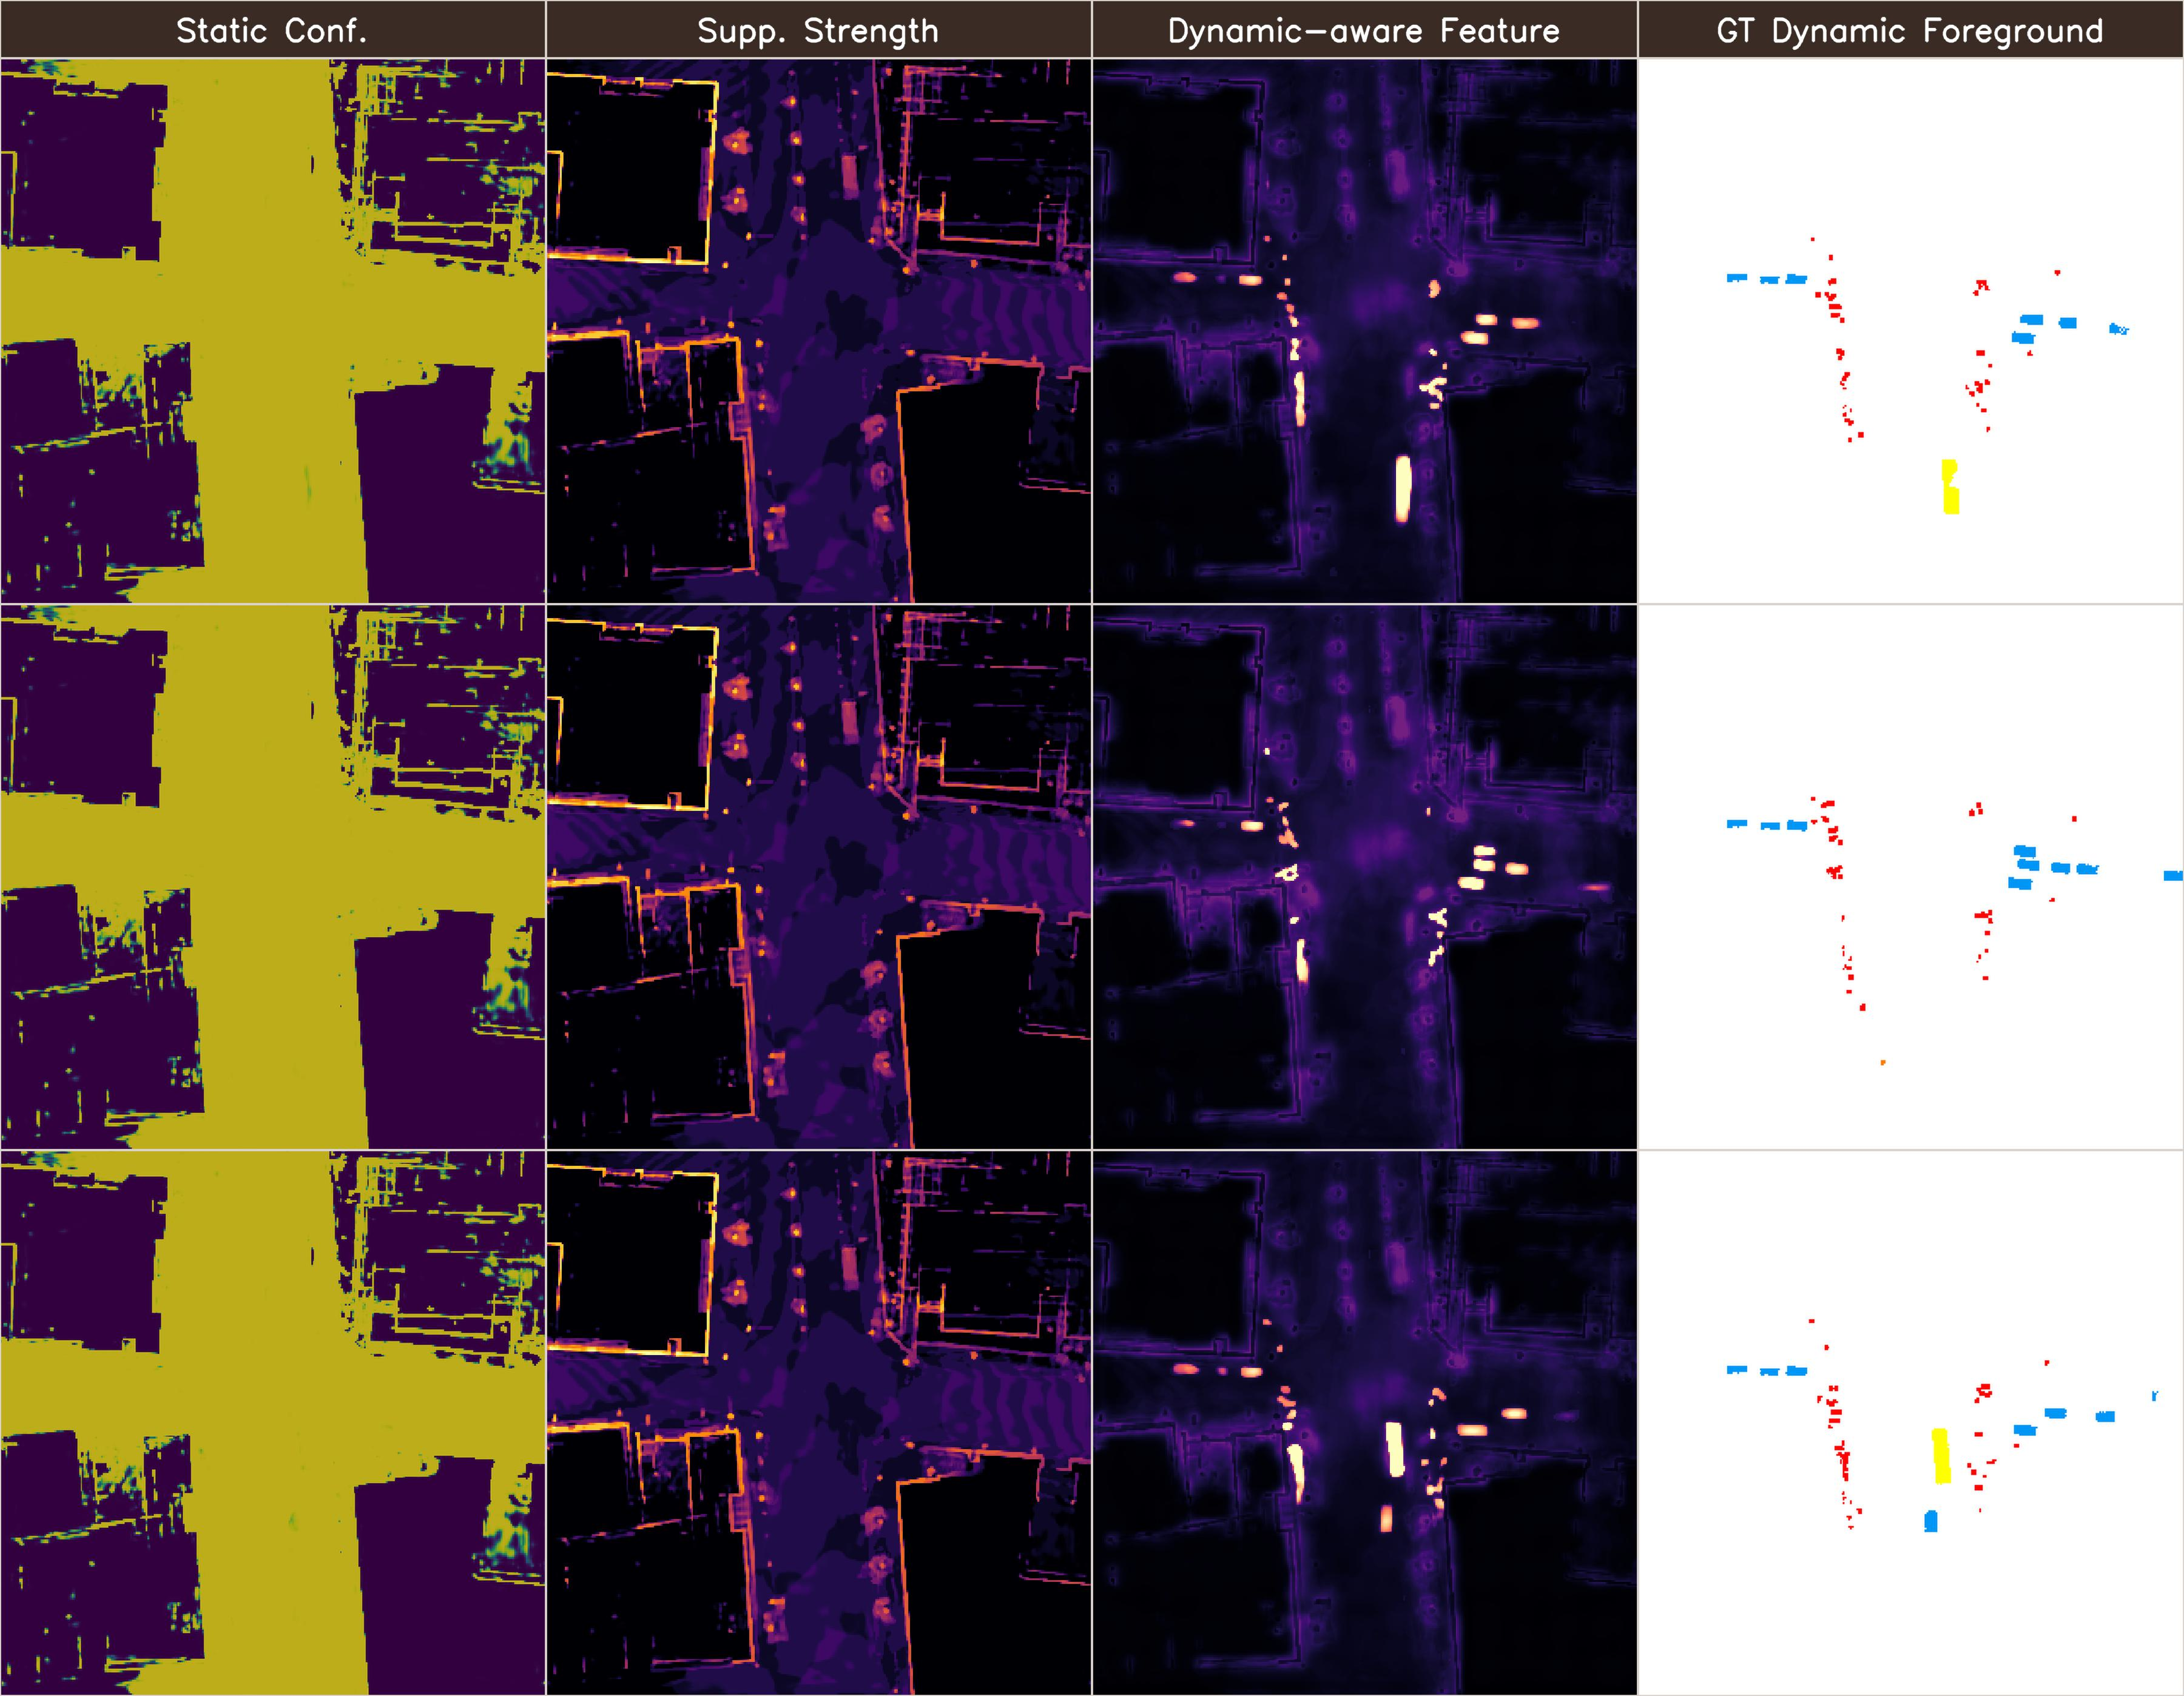
\includegraphics[width=\columnwidth]{figures/fig10-prosd-mechanism-features.pdf}
  \caption{\textbf{Progressive static-to-dynamic feature visualization.}
  Each row shows one validation sample. The columns visualize static
  confidence, static-confidence suppression strength, the Dynamic-aware
  feature (visualized as dynamic-enhanced feature energy with low-contrast
  scene context after static suppression), and the corresponding ground-truth
  dynamic foreground occupancy cropped from the full occupancy map.}
  \label{fig:prosd_mechanism_features}
\end{figure}

\begin{table}[!tbp]
\caption{\textbf{Core ablation of progressive static-to-dynamic reasoning.} The upper block compares prediction paradigms; the lower block isolates suppression and raw-feature bypass. The parallel S2D control uses the same no-static-suppression setting as the lower-block control.}
\label{tab:core_mechanism}
\centering
\scriptsize
\setlength{\tabcolsep}{4.2pt}
\renewcommand{\arraystretch}{1.08}
\begin{tabularx}{\columnwidth}{@{}>{\raggedright\arraybackslash}Xcccc@{}}
\toprule
Setting & gIoU$\uparrow$ & $\mathrm{mIoU}_{\mathrm{all}}\uparrow$ & $\mathrm{mIoU}_{\mathrm{dyn}}\uparrow$ & $\mathrm{mIoU}_{\mathrm{sta}}\uparrow$ \\
\midrule
\multicolumn{5}{l}{\textbf{\textit{Necessity of Progressive S2D Reasoning}}} \\
Plain Occupancy Prediction & 78.54 & 50.71 & 23.48 & 71.14 \\
Parallel S2D Fusion (no supp.) & 79.77 & 53.59 & 24.43 & 75.46 \\
Progressive S2D Reasoning & 89.08 & 60.08 & 28.97 & 83.42 \\
\midrule
\multicolumn{5}{l}{\textbf{\textit{Design of Progressive S2D Reasoning}}} \\
No static suppression & 79.77 & 53.59 & 24.43 & 75.46 \\
Suppression only & 88.35 & 59.77 & 28.81 & 82.99 \\
Suppression + raw bypass & 89.08 & 60.08 & 28.97 & 83.42 \\
\bottomrule
\end{tabularx}
\end{table}

\noindent \textbf{Protocol.}
The experiments are organized around three questions aligned with the paper's
claims: whether \nameplus{} improves infrastructure occupancy across sensing
regimes, which components cause the gain, and where the model remains
sensitive under harder diagnostic settings. All main comparisons are conducted
on InfraOcc under camera-only (C), LiDAR-only (L), and multi-modal (C+L)
tracks, using the official test split and the same voxel label space. Controlled
ablations are reported under the camera-only setting because depth evidence is
weakest there and persistent static background cues are strongest; this setting
therefore isolates the effect of progressive static-to-dynamic reasoning
without hiding it behind LiDAR geometry. Unless otherwise stated, models are
trained for 36 epochs with the same resolution, voxel grid, augmentation,
optimizer, learning-rate schedule, and class weights.

\noindent \textbf{Metrics.}
We report geometric IoU (gIoU), semantic mIoU over non-free valid classes
(All), dynamic-class mIoU (Dyn.), static-class mIoU (Sta.), and free-space IoU.
These metrics serve different checks. All measures the final semantic occupancy
field, Dyn. directly measures sparse traffic participants, Sta. verifies that
dynamic gains are not obtained by damaging the persistent layout, and gIoU/free
space track geometric occupancy quality. Dynamic classes are bicycle, bus, car,
motorcycle, pedestrian, and truck. Static classes are others, barrier,
traffic cone, driveable surface, sidewalk, terrain, manmade, and vegetation;
construction vehicle, trailer, other flat, and free space are excluded from all
mIoU means. Thus, $\mathrm{mIoU}_{\mathrm{all}}=(6\,\mathrm{mIoU}_{\mathrm{dyn}}
+8\,\mathrm{mIoU}_{\mathrm{sta}})/14$. Because the core difficulty of fixed roadside
occupancy is that dynamic participants are easily absorbed by stable
background, Dyn. is the primary diagnostic metric in the analysis, while
All/Sta./gIoU are used to check that the improvement remains globally
consistent.

\subsection{Quantitative Results}
\subsubsection{Main Comparison}
\begin{table}[!tbp]
\caption{\textbf{Static guidance quality.} Only the guidance signal for residual modulation is changed.
None uses the shared no-static-suppression control, Noisy uses a perturbed static-confidence map,
Predicted uses learned static confidence from static branch, and Oracle
uses ground-truth static occupancy as guidance.}
\label{tab:static_guidance_quality}
\centering
\scriptsize
\setlength{\tabcolsep}{2.8pt}
\renewcommand{\arraystretch}{1.08}
\begin{tabular*}{\columnwidth}{@{\extracolsep{\fill}}lcccc@{}}
\toprule
Guidance & gIoU$\uparrow$ & $\mathrm{mIoU}_{\mathrm{all}}\uparrow$ & $\mathrm{mIoU}_{\mathrm{dyn}}\uparrow$ & $\mathrm{mIoU}_{\mathrm{sta}}\uparrow$ \\
\midrule
None & 79.77 & 53.59 & 24.43 & 75.46 \\
Noisy & 86.70 & 56.51 & 22.60 & 81.95 \\
Predicted & 89.08 & 60.08 & 28.97 & 83.42 \\
Oracle & 89.22 & 60.31 & 29.18 & 83.65 \\
\bottomrule
\end{tabular*}
\end{table}

\begin{table}[!tbp]
\caption{\textbf{Suppression strength design.} We compare static-guided attenuation choices and initialization sensitivity.}
\label{tab:suppression_strength}
\centering
\scriptsize
\setlength{\tabcolsep}{2.3pt}
\renewcommand{\arraystretch}{1.08}
\begin{tabular*}{\columnwidth}{@{\extracolsep{\fill}}lccccc@{}}
\toprule
Setting & $\alpha_{\mathrm{init}}$ & gIoU$\uparrow$ & $\mathrm{mIoU}_{\mathrm{all}}\uparrow$ & $\mathrm{mIoU}_{\mathrm{dyn}}\uparrow$ & $\mathrm{mIoU}_{\mathrm{sta}}\uparrow$ \\
\midrule
\multicolumn{6}{l}{\textbf{\textit{Necessity of learnable suppression}}} \\
No static suppression & 0.0 & 79.77 & 53.59 & 24.43 & 75.46 \\
Fixed suppression & 0.5 & 84.30 & 56.68 & 28.32 & 77.95 \\
Learnable suppression & 0.5 & 89.08 & 60.08 & 28.97 & 83.42 \\
\midrule
\multicolumn{6}{l}{\textbf{\textit{Sensitivity to initialization}}} \\
Learnable ($\alpha_{\mathrm{init}}=0.25$) & 0.25 & 86.42 & 58.27 & 28.72 & 80.44 \\
Learnable ($\alpha_{\mathrm{init}}=0.50$) & 0.50 & 89.08 & 60.08 & 28.97 & 83.42 \\
Learnable ($\alpha_{\mathrm{init}}=0.75$) & 0.75 & 86.10 & 57.91 & 28.64 & 79.86 \\
\bottomrule
\end{tabular*}
\end{table}

\begin{table}[!tbp]
\caption{\textbf{Adaptive fusion design.} The upper block tests learned routing; the lower block varies gate inputs and routing granularity.}
\label{tab:adaptive_fusion_design}
\centering
\scriptsize
\setlength{\tabcolsep}{2.2pt}
\renewcommand{\arraystretch}{1.08}
\begin{tabular*}{\columnwidth}{@{\extracolsep{\fill}}lcccc@{}}
\toprule
Setting & gIoU$\uparrow$ & $\mathrm{mIoU}_{\mathrm{all}}\uparrow$ & $\mathrm{mIoU}_{\mathrm{dyn}}\uparrow$ & $\mathrm{mIoU}_{\mathrm{sta}}\uparrow$ \\
\midrule
\multicolumn{5}{@{}l}{\textbf{\textit{Necessity of Adaptive Fusion}}} \\
Deterministic Average Merge & 86.34 & 58.29 & 27.72 & 81.22 \\
Deterministic Group-wise Merge & 86.98 & 58.75 & 28.04 & 81.78 \\
Adaptive Group-wise Fusion & 89.08 & 60.08 & 28.97 & 83.42 \\
\midrule
\multicolumn{5}{@{}l}{\textbf{\textit{Design of Adaptive Fusion}}} \\
Confidence-only (group-wise) & 86.72 & 58.56 & 27.81 & 81.63 \\
Probability-only (group-wise) & 87.26 & 58.95 & 28.18 & 82.03 \\
Prob.+Conf. (class-wise) & 88.18 & 59.44 & 28.55 & 82.61 \\
Prob.+Conf. (group-wise) & 89.08 & 60.08 & 28.97 & 83.42 \\
\bottomrule
\end{tabular*}
\end{table}


Table~\ref{tab:infraocc_main_results} first establishes the main effectiveness
claim. In the camera-only track, where static background dominance is most
severe, \nameplus{} raises All from 50.71 to 60.08 and Dyn. from 23.48 to
28.97 over the plain camera baseline. The same comparison also improves Sta.
from 71.14 to 83.42 and gIoU from 78.54 to 89.08. The simultaneous gains in
Dyn., Sta., and gIoU are important for the paper's thesis: \nameplus{} does not
obtain better mIoU by simply fitting the persistent background, and it does not
recover dynamic objects by sacrificing layout quality.

The LiDAR-only and multi-modal tracks show that the same reasoning head remains
beneficial when stronger geometric evidence is available. \nameplus{} reaches
63.66/33.87 All/Dyn. in the L setting and 65.87/37.92 in the C+L setting,
outperforming the corresponding listed baselines in both overall and dynamic
occupancy. The lower camera-only Dyn. score reflects the difficulty of
monocular roadside depth inference, while the consistent ranking across C, L,
and C+L indicates that the contribution is not tied to one sensor front-end.
Instead, the gain comes from organizing voxel evidence from persistent static
layout toward residual dynamic occupancy.
\Cref{fig:infraocc_modality_qualitative} gives a sample-aligned qualitative
view of camera-based methods, placing roadside camera evidence, ground-truth
occupancy, and predictions from TPVFormer, SparseOCC, STCOcc, and \nameplus{}
(C) on each row. Compared with STCOcc, the progressive camera model is less
affected by the dominant static road layout and recovers a cleaner occupancy
field.
\begin{figure}[!t]
  \centering
  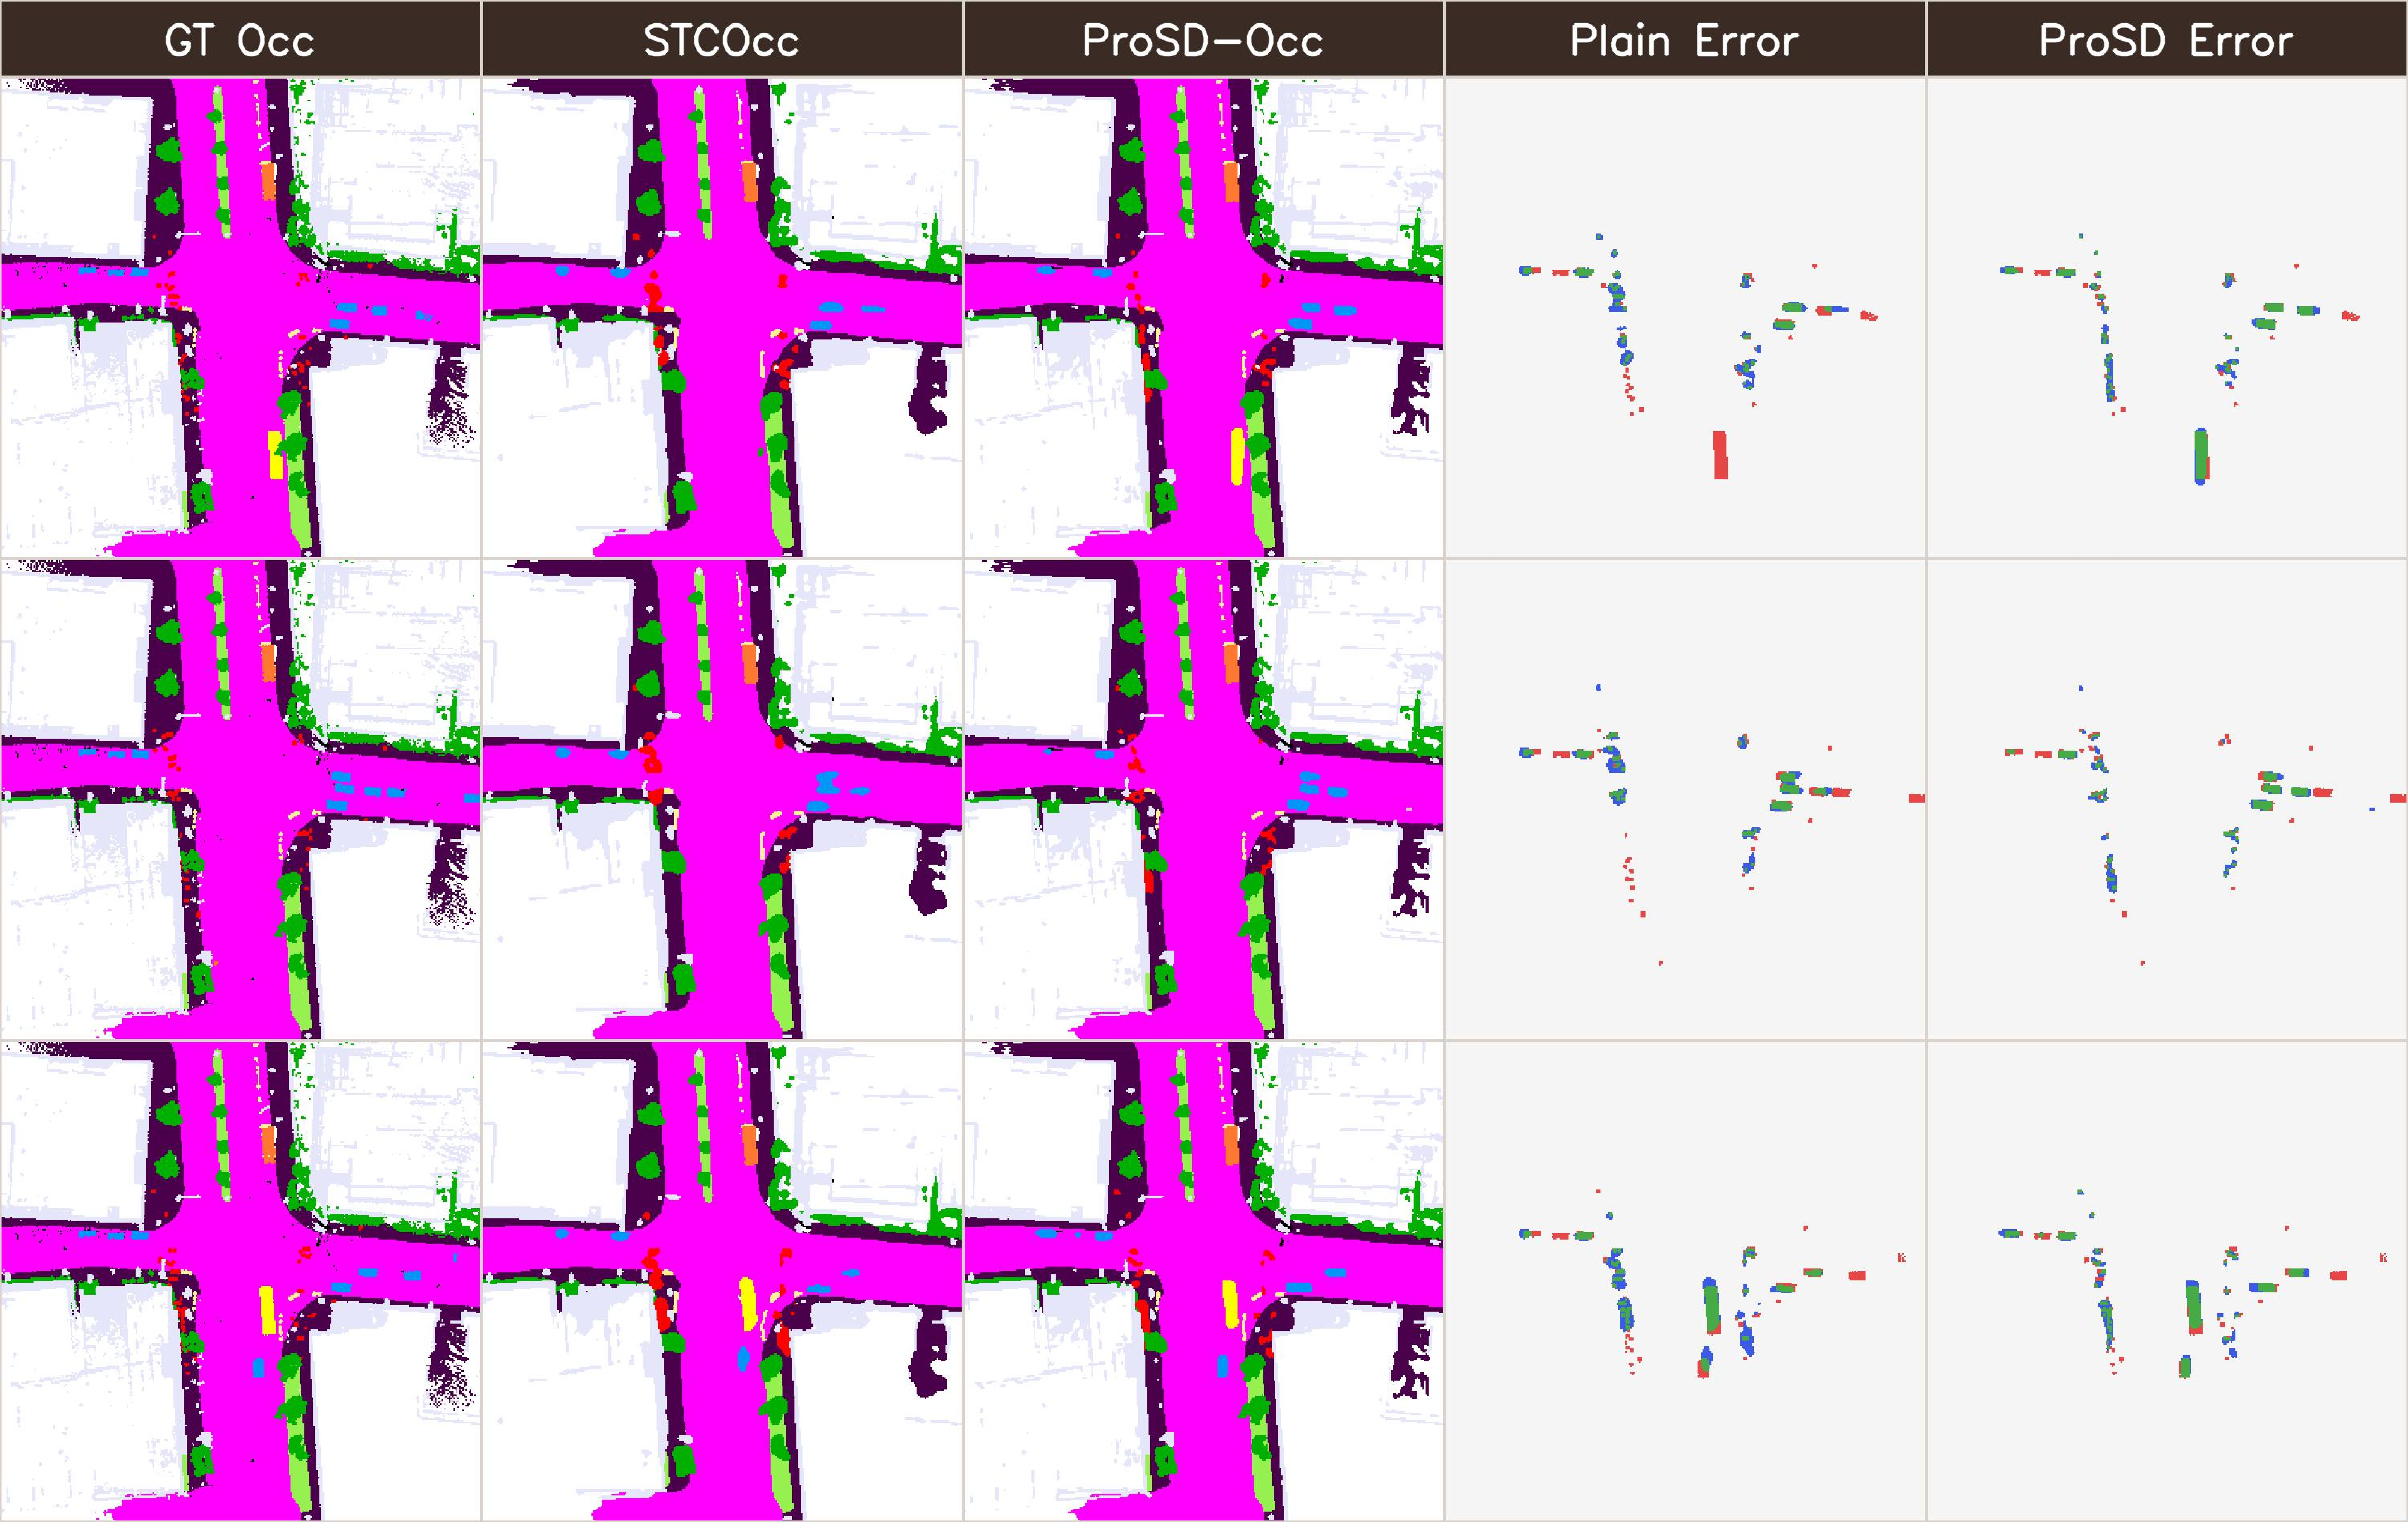
\includegraphics[width=\columnwidth]{figures/fig11-prosd-mechanism-errors.pdf}
  \caption{\textbf{Dynamic occupancy recovery by progressive reasoning.}
  Each row uses the same sample as \Cref{fig:prosd_mechanism_features}.
  STCOcc denotes the Plain (C) baseline. The error maps compare dynamic
  foreground occupancy only: green indicates correct dynamic prediction, blue
  indicates missed dynamic occupancy, and red indicates false dynamic
  prediction.}
  \label{fig:prosd_mechanism_errors}
\end{figure}

\begin{table}[!tbp]
\caption{\textbf{Static consistency ablation.} We test whether a stable layout regularizer improves progressive reasoning. Pairwise agreement is the default consistency form.}
\label{tab:static_consistency}
\centering
\scriptsize
\setlength{\tabcolsep}{2.8pt}
\renewcommand{\arraystretch}{1.08}
\begin{tabular*}{\columnwidth}{@{\extracolsep{\fill}}lcccc@{}}
\toprule
Setting & gIoU$\uparrow$ & $\mathrm{mIoU}_{\mathrm{all}}\uparrow$ & $\mathrm{mIoU}_{\mathrm{dyn}}\uparrow$ & $\mathrm{mIoU}_{\mathrm{sta}}\uparrow$ \\
\midrule
\multicolumn{5}{l}{\textbf{\textit{Necessity of Static Consistency}}} \\
No consistency & 86.10 & 58.34 & 28.20 & 80.95 \\
Static consistency (default) & \bestcell{89.08} & \bestcell{60.08} & \bestcell{28.97} & \bestcell{83.42} \\
\midrule
\multicolumn{5}{l}{\textbf{\textit{Design of Static Consistency}}} \\
Pairwise agreement & \bestcell{89.08} & \bestcell{60.08} & \bestcell{28.97} & \bestcell{83.42} \\
Batch-level consensus & 88.83 & 59.81 & 28.74 & 83.12 \\
\bottomrule
\end{tabular*}
\end{table}

\begin{table}[!tbp]
\caption{\textbf{Static--dynamic loss balance.} We vary branch coefficients while keeping the model architecture fixed.}
\label{tab:loss_balance}
\centering
\scriptsize
\setlength{\tabcolsep}{2.6pt}
\renewcommand{\arraystretch}{1.08}
\begin{tabular*}{\columnwidth}{@{\extracolsep{\fill}}lcccccc@{}}
\toprule
Setting & $\lambda_{\mathrm{sta}}$ & $\lambda_{\mathrm{dyn}}$ & gIoU$\uparrow$ & $\mathrm{mIoU}_{\mathrm{all}}\uparrow$ & $\mathrm{mIoU}_{\mathrm{dyn}}\uparrow$ & $\mathrm{mIoU}_{\mathrm{sta}}\uparrow$ \\
\midrule
Static-light  & 0.5 & 1.0 & 87.54 & 59.52 & 28.99 & 82.41 \\
Dynamic-light & 1.0 & 0.5 & 87.96 & 59.37 & 27.63 & 83.18 \\
Balanced      & 1.0 & 1.0 & \bestcell{89.08} & \bestcell{60.08} & 28.97 & \bestcell{83.42} \\
Dynamic-heavy & 1.0 & 2.0 & 87.83 & 59.82 & \bestcell{29.26} & 82.74 \\
Static-heavy  & 2.0 & 1.0 & 88.34 & 59.46 & 27.72 & 83.27 \\
\bottomrule
\end{tabular*}
\end{table}

\begin{table}[!tbp]
\caption{\textbf{Occupancy loss components.} CE, semantic-scaling, and Lovasz terms are varied for each supervision target.}
\label{tab:loss_terms}
\centering
\scriptsize
\setlength{\tabcolsep}{1.2pt}
\renewcommand{\arraystretch}{1.08}
\begin{tabular*}{\columnwidth}{@{\extracolsep{\fill}}lccccccc@{}}
\toprule
Setting & CE & Sem. & Lovasz & gIoU$\uparrow$ & $\mathrm{mIoU}_{\mathrm{all}}\uparrow$ & $\mathrm{mIoU}_{\mathrm{dyn}}\uparrow$ & $\mathrm{mIoU}_{\mathrm{sta}}\uparrow$ \\
\midrule
\multicolumn{8}{l}{\textbf{\textit{Static occupancy supervision}}} \\
CE only & \cmark &  &  & 86.80 & 58.48 & 26.89 & 82.18 \\
CE + Sem. & \cmark & \cmark &  & 87.89 & 59.22 & 27.08 & 83.33 \\
CE + Lovasz & \cmark &  & \cmark & 86.20 & 58.99 & 28.49 & 81.86 \\
CE + Sem. + Lovasz & \cmark & \cmark & \cmark & 89.08 & 60.08 & 28.97 & 83.42 \\
\midrule
\multicolumn{8}{l}{\textbf{\textit{Dynamic occupancy supervision}}} \\
CE only & \cmark &  &  & 86.78 & 57.33 & 25.49 & 81.21 \\
CE + Sem. & \cmark & \cmark &  & 87.54 & 58.33 & 27.34 & 81.57 \\
CE + Lovasz & \cmark &  & \cmark & 87.42 & 58.29 & 27.93 & 81.06 \\
CE + Sem. + Lovasz & \cmark & \cmark & \cmark & 89.08 & 60.08 & 28.97 & 83.42 \\
\midrule
\multicolumn{8}{l}{\textbf{\textit{Fusion-output occupancy supervision}}} \\
CE only & \cmark &  &  & 85.64 & 56.58 & 25.92 & 79.58 \\
CE + Sem. & \cmark & \cmark &  & 86.92 & 57.81 & 27.06 & 80.87 \\
CE + Lovasz & \cmark &  & \cmark & 86.56 & 57.56 & 27.47 & 80.13 \\
CE + Sem. + Lovasz & \cmark & \cmark & \cmark & 89.08 & 60.08 & 28.97 & 83.42 \\
\bottomrule
\end{tabular*}
\end{table}


\subsection{Ablation Studies}
\subsubsection{Progressive Static-to-Dynamic Reasoning}
Table~\ref{tab:core_mechanism} tests the central causal claim: dynamic
occupancy improves when the model reasons through static layout before
predicting residual objects. The flat baseline achieves 50.71 All and 23.48
Dyn. The parallel S2D/no-suppression control is the same
setting as the no-static-suppression row, reaching 53.59 All and 24.43 Dyn.;
this limited gain shows that independent static--dynamic prediction is not
sufficient without residual conditioning.
Progressive reasoning further reaches 60.08 All and 28.97 Dyn. because the
dynamic branch no longer competes with the full static scene in one step; it
receives a layout-conditioned feature where residual object evidence is easier
to recover.

The lower block explains why this residual feature must preserve both
suppressed and raw evidence. Static-guided suppression exposes dynamic cues and
improves Dyn. from 24.43 to 28.81, but suppression alone weakens the information
needed for complete semantic reconstruction. Adding the raw-feature bypass
produces the full result, raising Sta. to 83.42 while keeping the best Dyn.
This supports the intended role of the module: static evidence is not removed;
it is attenuated where it dominates and then recombined with residual evidence.
\Cref{fig:prosd_mechanism_features} visualizes the same mechanism across
multiple samples. Static confidence is high on persistent road and
infrastructure regions, suppression is applied around static-dominant
responses, and the Dynamic-aware feature, visualized as weighted branch-feature
energy, remains spatially continuous while emphasizing sparse foreground
occupancy. The last column shows the corresponding ground-truth dynamic
foreground to make the sparse target regions explicit.


\Cref{fig:prosd_mechanism_errors} then compares STCOcc, i.e., the
Plain (C) baseline, with \nameplus{} (C). The error maps show that residual
modulation reduces missed and false dynamic occupancy without turning the static
branch into a memorized background mask.

\begin{figure}[!t]
  \centering
  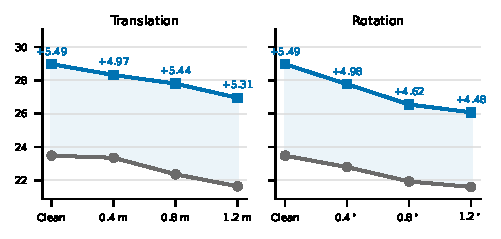
\includegraphics[width=\columnwidth]{figures/fig12-robustness-curves.pdf}
  \caption{\textbf{Robustness difference between \nameplus{} (C) and Plain (C).}
  The two panels report absolute dynamic mIoU under translation and rotation
  re-anchoring. Gray circles denote Plain (C), blue squares denote
  \nameplus{} (C), and the numbers above each setting denote
  \nameplus{} (C) minus Plain (C).}
  \label{fig:robustness_c_prosd_vs_plain}
\end{figure}

\begin{table}[!t]
\caption{\textbf{Accuracy--efficiency comparison.} Parameters and latency are measured from reproduced local configurations.}
\label{tab:capacity_efficiency}
\centering
\scriptsize
\setlength{\tabcolsep}{2.1pt}
\renewcommand{\arraystretch}{1.08}
\begin{tabular*}{\columnwidth}{@{\extracolsep{\fill}}lcccc@{}}
\toprule
Setting & Params. (M)$\downarrow$ & Lat. (ms)$\downarrow$ & $\mathrm{mIoU}_{\mathrm{all}}\uparrow$ & $\mathrm{mIoU}_{\mathrm{dyn}}\uparrow$ \\
\midrule
\multicolumn{5}{l}{\textbf{\textit{End-to-end efficiency}}} \\
\multicolumn{5}{l}{\textit{Multi-modal (C+L)}} \\
% M-CONet~\cite{OpenOccupancy} & 108.10 & 167.08 & 57.23 & 34.78 \\
BEVFusion~\cite{BEVFusion} & 108.01 & 103.73 & 55.44 & 32.57 \\
% BEVDepth~\cite{BEVDepth} & 108.01 & 150.36 & 55.34 & 33.07 \\
M-ProSD-Occ & 87.02 & 164.42 & 65.87 & 37.92 \\
\midrule
\multicolumn{5}{l}{\textit{LiDAR-only (L)}} \\
% L-CONet~\cite{OpenOccupancy} & 73.27 & 227.34 & 57.76 & 32.48 \\
VoxelNet~\cite{VoxelNet} & 73.25 & 75.43 & 53.87 & 31.13 \\
PointPillars~\cite{PointPillars} & 11.59 & 61.68 & 50.51 & 31.55 \\
L-ProSD-Occ & 30.24 & 109.55 & 63.66 & 33.87 \\
\midrule
\multicolumn{5}{l}{\textit{Camera-only (C)}} \\
BEVDet~\cite{BEVDet} & 100.66 & 41.92 & 45.14 & 21.19 \\
BEVFormer~\cite{BEVFormer} & 69.21 & 180.59 & 47.76 & 10.73 \\
BEVDepth~\cite{BEVDepth} & 100.66 & 57.43 & 46.81 & 19.64 \\
TPVFormer~\cite{TPVFormer} & 80.76 & 134.63 & 43.09 & 4.36 \\
SurroundOcc~\cite{SurroundOcc} & 80.04 & 44.40 & 50.77 & 11.37 \\
CONet~\cite{OpenOccupancy} & 100.74 & 53.23 & 49.25 & 18.93 \\
% STCOcc~\cite{STCOcc} & 59.33 & 178.55 & 50.71 & 23.48 \\
SparseOcc~\cite{SparseOcc} & 105.08 & 64.30 & 45.42 & 9.41 \\
GaussianFormer~\cite{GaussianFormer} & 36.32 & 65.50 & 43.63 & 10.45 \\
C-ProSD-Occ & 57.65 & 72.06 & 60.08 & 28.97 \\
\bottomrule
\end{tabular*}
\end{table}

\subsubsection{Guidance, Suppression, and Recomposition}
Tables~\ref{tab:static_guidance_quality}--\ref{tab:adaptive_fusion_design}
decompose the residual recovery path into guidance, attenuation, and
recomposition. Table~\ref{tab:static_guidance_quality} shows that static
guidance is necessary and that its quality matters. With
guidance disabled, the row uses the shared no-static-suppression control
reported in Tables~\ref{tab:core_mechanism} and~\ref{tab:suppression_strength},
giving 53.59 All and 24.43 Dyn. Noisy guidance further harms dynamic
prediction, and learned static confidence reaches 28.97 Dyn., close to oracle
guidance. Thus the static
branch is not just an auxiliary supervision head; it provides a sample-adaptive
soft explanation of persistent layout that makes residual dynamic evidence
easier to locate.

Table~\ref{tab:suppression_strength} shows that the attenuation should be
learned rather than fixed. Fixed suppression improves Dyn. over no suppression,
from 24.43 to 28.32, confirming that static confidence is useful as a soft mask
for exposing residual foreground cues. However, a fixed gate cannot adapt to
scene-dependent ambiguity and remains limited in All/Sta. In contrast,
learnable suppression raises All/Sta. to 60.08/83.42 while also giving the best
Dyn. among practical settings. The initialization study reinforces the same
interpretation: both weaker ($\alpha_{\mathrm{init}}=0.25$) and stronger
($\alpha_{\mathrm{init}}=0.75$) starting points preserve reasonable Dyn., but
they reduce All and Sta. This indicates that the gate must balance residual
mining and layout preservation, rather than simply maximizing foreground
response or suppressing static features aggressively.

Table~\ref{tab:adaptive_fusion_design} then verifies the final recomposition
step. The differences are moderate rather than dominant:
deterministic average and deterministic group-wise merging trail the default by
1.79 and 1.33 All, respectively, showing that fixed recomposition is
suboptimal but not catastrophic. One-input gates also lose about 1.1--1.5 All,
while class-wise routing remains closer to the default but still weakens
All/Sta. This pattern is consistent with adaptive fusion being an auxiliary
recomposition design: it stabilizes the final static/dynamic routing, but the
main improvement still comes from progressive residual reasoning.


\begin{table}[!tbp]
\caption{\textbf{Distance-wise dynamic occupancy performance.} Dynamic mIoU is evaluated in BEV distance intervals from the infrastructure sensor origin.}
\label{tab:distance_robustness}
\centering
\scriptsize
\setlength{\tabcolsep}{3.6pt}
\renewcommand{\arraystretch}{1.08}
\begin{tabular*}{\columnwidth}{@{\extracolsep{\fill}}lccc@{}}
\toprule
Setting & \multicolumn{3}{c}{$\mathrm{mIoU}_{\mathrm{dyn}}\uparrow$} \\
\cmidrule(lr){2-4}
& 0--20\,m & 20--40\,m & 40--60\,m \\
\midrule
ProSD-Occ (C) & 29.66 & 31.90 & 8.24 \\
ProSD-Occ (L) & 35.36 & 34.08 & 21.22 \\
ProSD-Occ (C+L) & 37.58 & 39.60 & 23.28 \\
\bottomrule
\end{tabular*}
\end{table}

\begin{table}[!tbp]
\caption{\textbf{Robustness to static-background overfitting.} We re-anchor the
test ego frame with controlled translations or yaw rotations while keeping the
physical scene unchanged, so coordinate-specific static-background shortcuts
become unreliable. Each entry reports $\mathrm{mIoU}_{\mathrm{dyn}}$.}
\label{tab:background_overfitting}
\centering
\scriptsize
\setlength{\tabcolsep}{2.2pt}
\renewcommand{\arraystretch}{1.08}
\begin{tabularx}{\columnwidth}{@{}>{\raggedright\arraybackslash}X C{1.08cm}C{1.08cm}C{1.08cm}C{1.08cm}@{}}
\toprule
Setting & \multicolumn{4}{c}{$\mathrm{mIoU}_{\mathrm{dyn}}\uparrow$} \\
\cmidrule(lr){2-5}
& Clean & 0.4\,m & 0.8\,m & 1.2\,m \\
\midrule
\multicolumn{5}{l}{\textbf{\textit{Translation re-anchoring}}} \\
STCOcc~\cite{STCOcc} & 23.48 & 23.35 & 22.36 & 21.64 \\
ProSD-Occ (C) & 28.97 & 28.32 & 27.80 & 26.95 \\
ProSD-Occ (L) & 33.87 & 31.05 & 27.70 & 29.34 \\
ProSD-Occ (C+L) & 37.92 & 36.42 & 33.51 & 33.91 \\
\midrule
Setting & \multicolumn{4}{c}{$\mathrm{mIoU}_{\mathrm{dyn}}\uparrow$} \\
\cmidrule(lr){2-5}
& Clean & $0.4^\circ$ & $0.8^\circ$ & $1.2^\circ$ \\
\midrule
\multicolumn{5}{l}{\textbf{\textit{Rotation re-anchoring}}} \\
STCOcc~\cite{STCOcc} & 23.48 & 22.79 & 21.93 & 21.60 \\
ProSD-Occ (C) & 28.97 & 27.77 & 26.55 & 26.08 \\
ProSD-Occ (L) & 33.87 & 32.43 & 32.27 & 25.92 \\
ProSD-Occ (C+L) & 37.92 & 36.20 & 34.40 & 28.85 \\
\bottomrule
\end{tabularx}
\end{table}


\subsubsection{Static Consistency}
Table~\ref{tab:static_consistency} checks whether the static scaffold used for
residual modulation should be regularized across samples. Removing consistency
reduces All from 60.08 to 58.34 and Sta. from 83.42 to 80.95, and also lowers
Dyn. from 28.97 to 28.20. In the design block, pairwise agreement is the
default consistency form and therefore matches the static-consistency row.
Batch-level consensus remains close but is slightly weaker at 59.81 All, 28.74
Dyn., and 83.12 Sta., indicating that broader batch aggregation can smooth out
sample-specific static details. The final model therefore keeps pairwise
agreement as the default static regularizer.

\subsubsection{Loss Design}
Table~\ref{tab:loss_balance} checks whether the dynamic gain could be obtained
by loss reweighting alone. Dynamic-heavy training gives the highest Dyn.
(29.26), but its All and Sta. are lower than the balanced setting. Conversely,
dynamic-light or static-heavy settings preserve more layout structure but
weaken dynamic recovery. The balanced objective is therefore used because it
best supports the coupled roles of the two branches: static layout explains the
persistent scaffold, while dynamic supervision recovers sparse residual
objects.

Table~\ref{tab:loss_terms} studies the loss terms used for each supervision
target. CE alone provides category supervision but is insufficient under the
severe static-dynamic imbalance of roadside scenes. Semantic scaling improves
calibration under class imbalance, and Lovasz improves region-level overlap for
fragmented dynamic objects. The full CE+Sem.+Lovasz setting gives the strongest
branch results, while the fusion-output block confirms that the final
recomposed occupancy field also needs structured supervision rather than a
single voxel-wise classification loss.

\subsection{Further Analysis}
\subsubsection{Efficiency}

Table~\ref{tab:capacity_efficiency} shows that the gain is not a consequence
of indiscriminate model scaling. In the camera-only setting, C-ProSD-Occ uses
fewer parameters than BEVDet, BEVDepth, SparseOcc, and CONet, while achieving
the best All and Dyn. among the listed methods. In the LiDAR-only and
multi-modal settings, the method also remains competitive in parameter count
while giving substantially stronger occupancy accuracy. These results match the
contribution of the paper: \nameplus{} changes how voxel evidence is organized
at the decision stage, rather than relying on a larger feature extractor.

\subsubsection{Distance-wise Dynamic Occupancy}

Table~\ref{tab:distance_robustness} evaluates where dynamic occupancy remains
difficult after the main gains. C-ProSD obtains 29.66 Dyn. in the 0--20\,m
range and 31.90 in the 20--40\,m range, but drops to 8.24 in the 40--60\,m
range. Adding explicit geometry improves the far-range bin substantially:
L-ProSD reaches 35.36/34.08/21.22 over the three distance bins, and M-ProSD
further reaches 37.58/39.60/23.28. This trend clarifies the scope of the
method. Progressive static-to-dynamic reasoning improves semantic organization
across sensing regimes, but long-range dynamic occupancy remains limited by the
available geometric evidence.

\subsubsection{Robustness to Static-Background Overfitting}
Table~\ref{tab:background_overfitting} tests a risk that is specific to
fixed-view infrastructure perception: a model may appear strong by associating
fixed coordinates with persistent background. We apply controlled rigid
ego-frame perturbations at test time by translating or yaw-rotating the
evaluation frame and applying the same re-anchoring to the sensor pose metadata
and labels. The physical scene is unchanged, but direct coordinate-background
shortcuts become less reliable. We therefore report dynamic mIoU after
re-anchoring: if dynamic recovery is driven by sensor evidence rather than
static-coordinate memorization, it should remain competitive when the static
scaffold is no longer aligned with its original coordinates.

The clean rows match the main-table plain and ProSD results. In the image-only
setting, C-ProSD starts from a stronger clean dynamic score and keeps higher
dynamic prediction than the plain baseline under all translation and rotation
perturbations. The L and C+L rows show the same absolute dynamic advantage
under most re-anchored settings, indicating that explicit geometry improves
dynamic evidence while remaining sensitive to coordinate-frame shifts.
\Cref{fig:robustness_c_prosd_vs_plain} makes this trade-off explicit by
plotting \nameplus{} (C) and Plain (C) as paired absolute dynamic-mIoU curves.
Across all tested translation and rotation shifts, the dynamic gap remains
positive, supporting the intended interpretation of ProSD reasoning: it improves
residual dynamic recovery from sensor evidence under controlled coordinate
re-anchoring.
